\section{Linear Regression}

Linear Regression is used a lot in statistics, where its primary purpose is to predict a target value based on independent predictors and is useful to find cause and effect relationships between variables \cite{linear_regression}. Before getting started on convolutional neural networks, we wanted to see if these problems were solvable with linear regression. The idea was to use the columns from the demographics dataset (see figure \ref{figure:demographics}). We did not expect high performance from this, as there are only 55 rows of participants. Anyone having a little bit of experience with machine learning will know that this is not nearly enough data. We wanted to do it regardless, to see how a linear regression model performed.

Not all of the columns are relevant though, for example, \textbf{number} is unique for each participant, so it does not make sense to use. The column \textbf{melanch} also does not make sense to use, as there is only one participant with Melancholia. \textbf{Inpatient} cannot be used because the participants in the control group are not patients, and cannot be either inpatient or outpatient. The same goes for \textbf{edu}, \textbf{work} and \textbf{marriage}, but we don't have these data values for control group participants. We don't have their \textbf{afftype} or any of the \textbf{MADRS} scores either, but we already know them: \textbf{afftype} should be 0 (not bipolar) and both \textbf{MADRS} scores should be 0 (not depressed). 

We used the \textbf{afftype} column as a target in the regression. This way we could classify whether a participant is in the control or the condition group, by setting the \textbf{afftype} value to either 0 or 1 instead of 0, 1, 2 or 3 (values above 1 reduced to 1), and ran the regression on all of the remaining columns one by one:

\begin{itemize}
      \item \textbf{Gender}
      \item \textbf{Age}
      \item \textbf{Days}
      \item \textbf{MADRS1}
      \item \textbf{MADRS2}
\end{itemize}

The model for this task is straightforward. We created a sequential model (source code in appendix \ref{code:regression_model}) with one input layer and one output layer. The input is a \textbf{dense} layer which takes one value (the value of the current column), activates using \textbf{relu} and outputs 5 neurons. In the output layer, we activate using a \textbf{linear} function (default activation function when none are specified) and return one value: the prediction. We compiled the model with the loss function \textbf{Mean Squared Error} and the optimizer \textbf{Adam}. 

Since we were predicting the \textbf{afftype} of a participant, which is a binary value (0 or 1) and a prediction from the model yields a value between 0 and 1, we rounded the prediction value to the nearest integer after running predictions on the test data. Doing it this way instead of making a classification model, makes the \textbf{loss} value more useful as a metric while training rather than accuracy. 

When testing the model, we wanted to achieve an accuracy of 100\% when using the \textbf{MADRS} scores. The task should be easy because of how easy it is using a simple check: if the MADRS score is 0, then the participant is in the control group. If not, the participant is in the condition group. We did not need to use machine learning on these columns but was interesting to train the model to find this relationship without telling it the simple rule. For the other columns, we did not know what to expect; maybe there was a relationship, maybe not.

\section{1D Convolutional Neural Network}

\subsection{Convolution}

\begin{figure}[h]
\begin{center}
    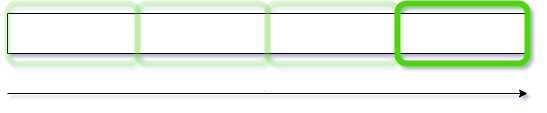
\includegraphics[height=2.5cm]{img/feature_detector.png}
    \caption{Feature Detector / Filter "sliding" over input data}
    \label{figure:feature_detector}
\end{center}
\end{figure}

\noindent The main ingredients in a CNN are \textit{convolutional} layers and \textit{pooling layers} \cite{deep_learning}. The convolutional layers are responsible for the convolution process, which in mathematics is a function derived from two given functions by integration which expresses how the shape of one is modified by the other \cite{convolution_definition}. 

The convolutional layer in machine learning consists of \textit{filters} \ref{figure:feature_detector}, which are the sliding windows that go through the input data.  They are also called \textit{feature detectors}, and using 100 of them means that the layer can detect 100 features. The size of a filter is called \textit{kernel size}. The output of the convolutional layer is a matrix with one column for each filter, and one row for each step in the convolution. How many steps there are, is given by the length of the input data (also called \textit{height}) minus the kernel size plus 1.

\subsection{Creating the Model}
\begin{figure}[!ht]
\begin{center}
      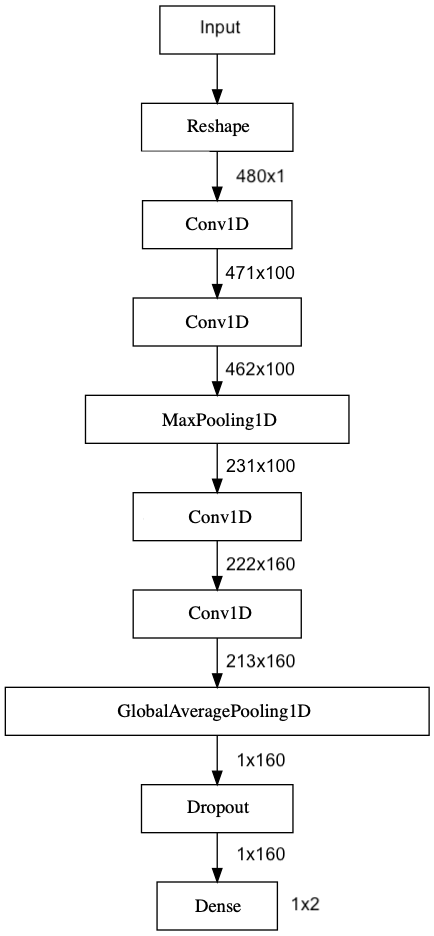
\includegraphics[height=19.5cm]{img/layers.png}
      \caption{The architecture of our convolutional neural network for the first objective. The segment length is 480 in this example. We can see the output shape underneath each layer.}
      \label{figure:layers}
\end{center}
\end{figure}

We built two convolutional neural network models. One model for the first two objectives was built for classification, and for the third objective we came up with another model built for prediction. To make a convolutional neural network, you need some \textit{convolutional} and \textit{pooling} layers. Which layers added in between and the ordering of them, together with the parameters passed to the layers, is what makes the model perform differently. 

\subsubsection{Classification}
The following model was used to achieve our first two objectives; classifying whether a participant belongs to the \textbf{control} or \textbf{condition} group, and classifying the participant's \textbf{depression class}. The only difference between these two objectives is the number of classes we are trying to classify, and therefore only the output layer needs to be changed. Full source code can be found in the appendix (\ref{code:1d_conv_net_classifier}).

\begin{enumerate}
      \item We started by defining a \textbf{Sequential} model. This is easy to understand and readable way of defining a model. Alternatively, we could have used a \textbf{functional} model, which would give more control of inputs and outputs of the layers. A \textbf{functional} model would also be useful if we wanted to debug and optimize each layer within the model. 
      
      \item \textbf{Reshape}: In the first layer we needed to reshape the input data so that it becomes an $X$ by 1 matrix, where $X$ is the length of each segment. The reason for the reshape step is because the next layer (\textbf{Conv1D}) requires the input to contain the parameters \textit{batch, steps and channels}. \textit{Batch} will be set to \textbf{None}, \textit{steps} will be the segments, and \textit{channels} will be $1$ (because we only have one measurement value for each minute).
      
      \item \textbf{Conv1D}: This is the first \textit{convolutional} layer, where the required parameters are how many \textit{filters} wanted, and how big the \textit{kernel} should be. We used 100 filters and a kernel size of 10. Having less or more filters might have an impact on the performance, but we did not want to over-complicate the model yet. There are many different parameters that we can use on a layer like this, for example, \textit{padding} and \textit{strides}, but using the default values was a good choice for now. The output of this layer results in a $(X-10+1) \times 100$ matrix, where $X$ is the length of each segment here as well. The activation function for all convolutional layers in this model is \textit{ReLU} (Rectified Linear Unit). 

      \item \textbf{Conv1D}: The second convolutional layer looks exactly like the first one, and the output is a $(X-10+1-10+1) \times 100$ matrix. 
      \item \textbf{MaxPooling1D}: Pooling is important in a convolutional neural network to reduce complexity, and its role is to merge semantically similar features into one \cite{deep_learning}. 
            \textit{Max pooling} works by reducing to only the maximum value for each \textit{window} of size $N \times N$. We used 2 as 
            window size ($N$), resulting in matrix that is half the size of the input: $ \frac{X-10+1-10+1}{2} \times 100$. 
            Pooling may also help reduce \textit{overfitting}, which is when the model learns its training data too well and performs worse on unseen data.
      \item \textbf{Conv1D}: Two more convolutional layers were added, and after these, the input to the next layer will be a matrix of size
            $ \left( \frac{X-10+1-10+1}{2}-10+1-10+1 \right) \times 160 $.
      \item \textbf{GlobalAveragePooling1D}: Another type of pooling layer was added, which takes the average of weights within the network instead of the maximum.
            The output of the \textit{global average pooling} layer is a matrix of size $ 1 \times 160 $.
      \item \textbf{Dropout}: A dropout layer is used to reduce overfitting, by randomly ignoring units in the neural network \cite{dropout}. 
      \item \textbf{Dense}: The final layer in the model is a dense layer (fully connected) which reduces the matrix from $160$ values to 
            either $2$ or $3$ (for objective one and two), with the activation function \textbf{softmax}. 
            Then the output (a $1$ in one of the neurons) is mapped to the corresponding label.
\end{enumerate}

\subsubsection{Prediction}
To make the model work for our third objective, where we predicted the value of participant's MADRS score, we had to change a few layers. We removed two of the \textit{Conv1D} layers and applied the following after the global average pooling layer:

\begin{enumerate}
      \setcounter{enumi}{7}
      \item \textbf{Flatten}: The matrix was required to be flat (one dimensional) before proceeding to the final layers.
      \item \textbf{Dense}: A dense layer with $10$ neurons was added, with \textit{ReLU} as the activation function. 
      \item \textbf{Dense}: The output layer is a dense layer of size $1$, because we are predicting \textit{one} value. 
            Also, the activation function is \textit{linear} instead of \textit{softmax}.
\end{enumerate}

Source code for this model can also be found in the appendix (\ref{code:1d_conv_net_predictor}).

\section{Optimizing the models}

\noindent Out of the box, we did not think that the models were going to perform perfectly. Therefore we needed to experiment with each parameter that we passed to the models and find the best ones. We had some ideas of what to change:

\begin{itemize}
    \item Use different segment lengths
    \item Tweak hyper-parameters
\end{itemize}

\noindent The first idea, using different segment lengths, was the one we thought was going to impact the results the most. Having more data inside each segment will give the neural network more opportunities to learn features, and then be better at its job of either classifying or predicting the outcome. Having longer segments also means that each epoch of training would take more time because each layer has to process more data. In chapter \ref{chapter:training}, we describe the process of finding the optimal segment lengths for each objective.

Hyper-parameters are all the \textit{higher-order} parameters we compile/train the model with. These are the bells and whistles of the learning algorithm \cite{hyperparameters}, and they are different from the parameters learned by training the model and need to be fixed for one session of model training. Finding the perfect ones can be crucial for a well-performing model. Hyper-parameters that we use in our models include:

\begin{itemize}
      \item \textbf{Optimizer and learning rate}\\
          The \textbf{optimizer} function (as discussed earlier) is essential to lower the loss value when fitting the dataset to the model. 
          Different optimizers have different input parameters, and the \textit{learning rate} is one that all optimizers use. 
          Tweaking the learning rate can yield better results, but the default learning rate for the chosen optimizer is always a good starting point because it is what the author of the optimizer set as default.
      \item \textbf{Epochs}\\
          Defines how many iterations of training that are to be executed, and in most cases more epochs yield better results up to a certain point.
      \item \textbf{Batch size}\\
          This is how much data that is processed at the same time each epoch, and the best batch size to use can be completely different on two different models. 
      \item \textbf{Train/test split size}\\
          When building a neural network, we want as much data as possible to both train and to test on afterward. We cannot use all the data in both cases, so the most balanced split needs to be determined.
\end{itemize}